\section{OmniEduBench}

Our proposed OmniEduBench education benchmark is designed as a \textcolor{myorange}{natively Chinese education evaluation benchmark} that captures the unique linguistic and cultural knowledge of Chinese education, encompasses diverse question types, and assesses LLMs not only on their knowledge capabilities but also on the distinctive cultivation competencies required in real-world educational scenarios. 

\subsection{Task Definition}

\textbf{Knowledge dimension} focuses on evaluating the model’s mastery of subject-specific knowledge. Tasks in this dimension include 11 common exam question types (\textit{e.g.}, multiple choice, multiple answer, fill-in-the-blank, short answer, composite questions, term explanation, True/False, calculation, logical reasoning, case analysis, and essay). These 11 question types span a wide range of disciplines, from humanities and history to science, engineering, and professional fields. The primary goal is to assess the LLM’s problem-solving capabilities within the context of real-world education. 

\textbf{Cultivation dimension} assesses LLMs on their ability to support holistic educational objectives beyond mere knowledge acquisition. This includes guiding students’ thinking processes, fostering moral and value development, enhancing emotional understanding, and promoting critical reasoning skills. Tasks in this dimension are designed to reflect realistic learning scenarios, where models must provide pedagogically sound feedback that aligns with students’ cognitive and emotional needs.

\begin{figure}[tbp]
    \centering
    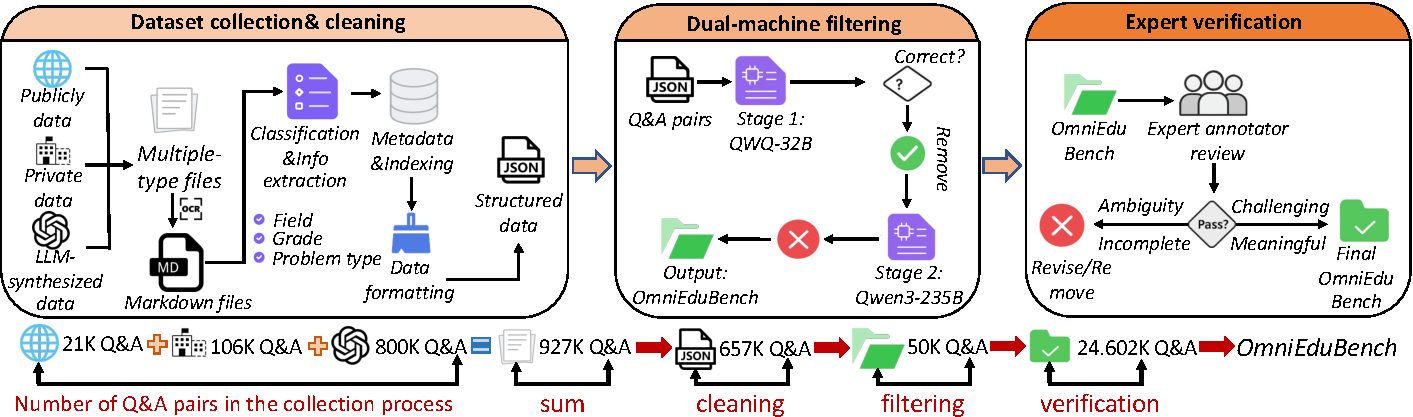
\includegraphics[height=0.3\textwidth]{figure/omniprocess.pdf}
    \vspace{-6mm}
    \caption{Overview of the construction process, including collection, cleaning, filtering, verification.}
    \label{fig:omniprocess}
    \vspace{-5mm}
\end{figure}

\subsection{Benchmark Construction}
\label{subsec:bc}

In this section, we provide a detailed overview of the construction process for the proposed OmniEduBench education evaluation benchmark, as illustrated in Figure~\ref{fig:omniprocess}. The process consists of four key stages: dataset collection, dataset cleaning, dual-machine filtering, and expert verification.

\textbf{Dataset collection.} OmniEduBench is designed to encompass a wide range of diverse scenarios to enable comprehensive evaluation. To achieve this, we employ three distinct data collection methods, carefully balancing diversity and efficiency in the construction of the OmniEduBench benchmark.

\textit{Manual collection of publicly available data.} 
Existing benchmarks often lack sufficient diversity in question types and knowledge coverage, making them inadequate for our 41 subjects in knowledge dimensions. To address this gap, we manually collected additional data from publicly available online resources (\textit{e.g.}, XuekeNet, ZujuanNet, ShijuanNet, ShitiNet) to enrich diversity and ensure coverage of underrepresented scenarios, such as primary and career education. Furthermore, guided by the Catalogue of Undergraduate Programs in Regular Higher Education Institutions~\footnote{\url{http://www.moe.gov.cn/srcsite/A08/moe_1034/s4930/202403/W020240319305498791768.pdf}} issued by China’s Ministry of Education, we curated a large body of review materials and exam questions across 13 academic disciplines, including philosophy, education, law, literature, history, science, engineering, agriculture, medicine, military science, management, and the arts. This effort significantly improves distributional balance and provides a more faithful reflection of real applications.

\textit{Manual collection of private data.}
Data contamination remains one of the most critical challenges in constructing evaluation datasets for LLMs. To mitigate this risk, we manually collected additional data from private resources, such as internal school exam papers. Unlike widely circulated national exams, these materials have never appeared on the public Internet or been included in large-scale web crawls, effectively reducing the risk of leakage. Incorporating such private data enhances the reliability and fairness of the benchmark, while providing a more rigorous assessment of models.

\textit{LLM-generated data.}
Given the difficulty of directly obtaining data in the cultivation dimension, we leveraged LLMs to generate a substantial number of scenario-based question–answer pairs, aiming to supplement gaps in existing resources. To ensure the quality of the synthetic data, we invited five education experts to conduct discussions on 20 cultivation subjects and consulted relevant books, papers, and other materials. The collected content was organized into a database, which was then provided to the LLM to enhance the fidelity and accuracy of the generated data. For generated questions, to increase their challenge, we designed highly confounding distractors via prompts and conducted sampling checks and revisions with expert verification (please see more details in expert verification). 
\textcolor{myorange}{Finally, we collected a total of 927K question–answer (Q\&A) pairs, including 21K from publicly available data, 106K from private data, and 800K generated by LLMs.}

\textbf{Dataset cleaning.}
The entire data cleaning process consists of multiple steps. (1) We used MinerU~\citep{wang2024mineru} to convert the collected 927K Q\&A pairs into Markdown (md) format, enabling structured management and efficient information extraction. (2) Detailed metadata were extracted for each question, including subject, grade level, question type, and knowledge tags, to construct comprehensive question profiles that facilitate data management and subsequent analysis. (3) Standard data cleaning procedures were applied, including deduplication, removal of questions with missing key content, filtering of sensitive or inappropriate content, and exclusion of questions that rely on external information.\textcolor{myorange}{After the cleaning process, we obtained a total of 657K Q\&A pairs.}

\begin{table}[tbp]
    \centering
    \caption{Statistics of OmniEduBench and more detailed per-subject information are shown in the Appendix. Bilingual names and abbreviations of six knowledge and six cultivation dimensions.}
    \vspace{0.2mm}
    \resizebox{0.99\textwidth}{!}{
    \begin{tabular}{lcc|lcc}
        \toprule
        \multicolumn{3}{c|}{\textcolor{myorange}{\textit{Knowledge dimension}}} & \multicolumn{3}{c}{\textcolor{myorange}{\textit{Cultivation dimension}}}\\
        English name & Abbreviation & Chinese name & English name & Abbreviation & Chinese name \\
        \midrule
        Law \& Politics  & LP &  \cc{法律与政治} & Character \& Values & CV & \cc{品格与价值观} \\ 
        Foundational Disciplines & FD & \cc{基础学科} & Personalized Development & PD & \cc{个性化发展} \\
        Humanities \& History & HH & \cc{人文与历史} & Social \& Interpersonal Skills & SIS & \cc{社会与人际交往} \\
        Medicine \& Health & MH & \cc{医学与健康}  & Thinking \& Cognitive Skills & TCS & \cc{思维与认知能力} \\
        Interdisciplinary \& Integrated Subjects & IIS & \cc{综合与交叉学科} &  Teaching Feedback \& Support & TFS & \cc{教学反馈与支持}) \\
        Social Sciences \& Economics Management & SSEM & \cc{社会科学与经济管理} & Emotional \& Mental Health & EMH & \cc{情感与心理健康} \\
        \bottomrule
    \end{tabular}}
%     \label{tab:name}
%     \vspace{-6mm}
% \end{table}
% \begin{table}[tbp]
%     \centering
%     \caption{Statistics of OmniEduBench with detailed per-subject information shown in the Appendix.}
%     \vspace{0.2mm}
    \resizebox{0.99\textwidth}{!}{
    \begin{tabular}{lcc|lcc|lcc}
        % \toprule
        Category & Subjects & Questions & Category & Subjects & Questions & Category & Subjects & Questions \\
        \midrule
        \multicolumn{3}{c|}{\textcolor{myorange}{\textit{In terms of dimension}}} & \multicolumn{3}{c|}{\textcolor{myorange}{\textit{In terms of Knowledge}}} & \multicolumn{3}{c}{\textcolor{myorange}{\textit{In terms of Cultivation}}} \\
        Knowledge  & 41 & 18,121 & LP & 4 & 1,455 & CV & 2 & 694 \\
        Cultivation & 20 & 6,481 & FD  & 11 & 7,918 & PD & 3 & 1,031 \\
        \multicolumn{3}{c|}{\textcolor{myorange}{\textit{In terms of different level}}} & HH & 10 & 5,331 & SIS & 3 & 736 \\
        K-12 Schools  & 10 & 4,384 & MH & 3 & 918 & TCS & 6 & 1,900 \\
        High school & 11 & 6,735 & IIS & 4 & 914 & TFS & 1 & 193 \\
        College  & 30 & 6,364 & SSEM & 9 & 1,643 & EMH & 5 & 1,833 \\
        \midrule
        Total  & 61 & 24,602 & Total  & 41 & 18,179 & Total  & 20 & 6,387 \\
        \bottomrule
    \end{tabular}}
    \label{tab:sta}
    \vspace{-6mm}
\end{table}

\textbf{Dual-machine filtering.}
To ensure OmniEduBench is a high-quality and challenging benchmark, we implemented a dual-model filtering mechanism on an \textcolor{myorange}{initial set of 657K Q\&A pairs}. Specifically, we first evaluated all questions using QWQ32B~\citep{qwq32b}, retaining only those that the model answered incorrectly. This initial filtering resulted in \textcolor{myorange}{a subset of 430K Q\&A pairs}. These questions then underwent a second filtering stage with the same strategy, this time using Qwen3-235B~\citep{yang2025qwen3}, ultimately yielding the final \textcolor{myorange}{set of 50K high-quality} and challenging data. 

\textbf{Expert verification.}
We recruited 50 master's students to perform an initial quality check on the dataset based on five predefined dimensions (as shown in Table~\ref{tab:ev}), removing any data that did not meet the criteria, which resulted in \textcolor{myorange}{a final set of 24.602K Q\&A pairs} for OmniEduBench. Subsequently, we invited 5 senior annotation experts to conduct a rigorous quality review on a 15\% random sample of the OmniEduBench. The review results, shown in Table~\ref{tab:ev}, indicate that the dataset maintains high overall quality, demonstrating both reliability and applicability.

\begin{table}[tbp]
    \centering
    \caption{Expert validation results for the OmniEduBench dataset.}
    \vspace{0.2mm}
    \resizebox{0.99\textwidth}{!}{
    \begin{tabular}{lcccc}
        \toprule
        Metric English name & Metric Chinese name & Average & Standard deviation & Inter-rater agreement  \\
        \midrule
        Overall quality & \cc{整体质量} & 4.8 & 0.1 & 0.90\\
        Clarity & \cc{问题清晰度} & 4.5 & 0.2 & 0.85 \\
        Option perplexity & \cc{选项困惑度} & 4.8 & 0.3 & 0.83 \\
        Accuracy & \cc{答案准确性} & 4.8 & 0.1 & 0.90 \\
        Cultivation value & \cc{育人价值} & 4.6 & 0.2 & 0.88 \\
        \bottomrule
    \end{tabular}}
    \label{tab:ev}
    \vspace{-6mm}
\end{table}

\subsection{Evaluation Criteria}
\label{subsec:ec}

Based on the characteristics of different question types, we adopt two evaluation metrics: (1) \textbf{Choice}. For questions with a standard answer, we directly evaluate the provided answer. This simplifies the scoring process, as the model only needs to select the most appropriate option, thereby reducing ambiguity in assessment. (2) \textbf{LLM-assisted scoring}. For short-answer questions that may have multiple valid forms but are semantically equivalent, we employ an LLM-assisted scoring method. This approach provides greater flexibility, avoids imposing unnecessary constraints on the model, and allows for a more accurate evaluation of the model’s semantic understanding and expression.

\subsection{Statistics}

Through rigorous data filtering and expert validation, we collected 18.121K high-quality question–answer pairs for the knowledge and 6.481K for the cultivation. As illustrated in Figure~\ref{fig:omniframe} and summarized in Table~\ref{tab:sta}, with more detailed per-subject statistics provided in the Appendix, the dataset spans 12 major categories, as shown in Table~\ref{tab:sta}, including K-12, higher school, university-level courses, and cultivation aspects such as emotion and reasoning, covering a total of 61 specific scenarios. Figures~\ref{fig:omni12} and~\ref{fig:omni34} present some representative examples in different dimensions and question types. The questions exhibit wide variability in type and difficulty and are sourced from diverse origins, primarily newly collected from public or private resources or manually constructed. 

\begin{figure}[tbp]
    \centering
    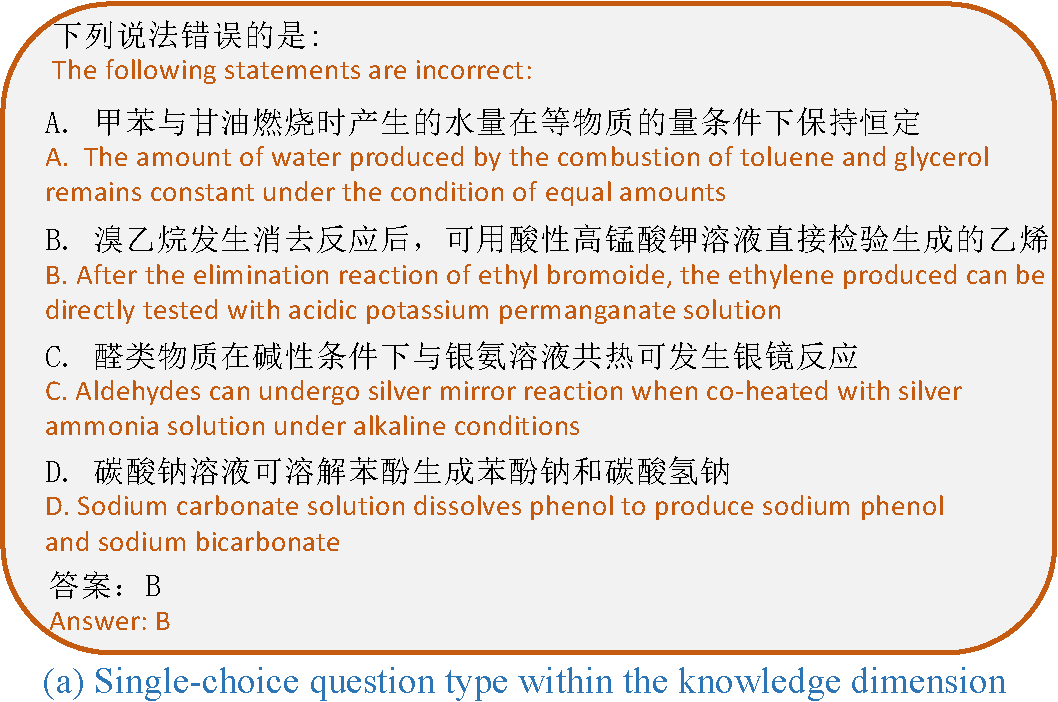
\includegraphics[height=0.32\textwidth]{figure/omni1.pdf}
    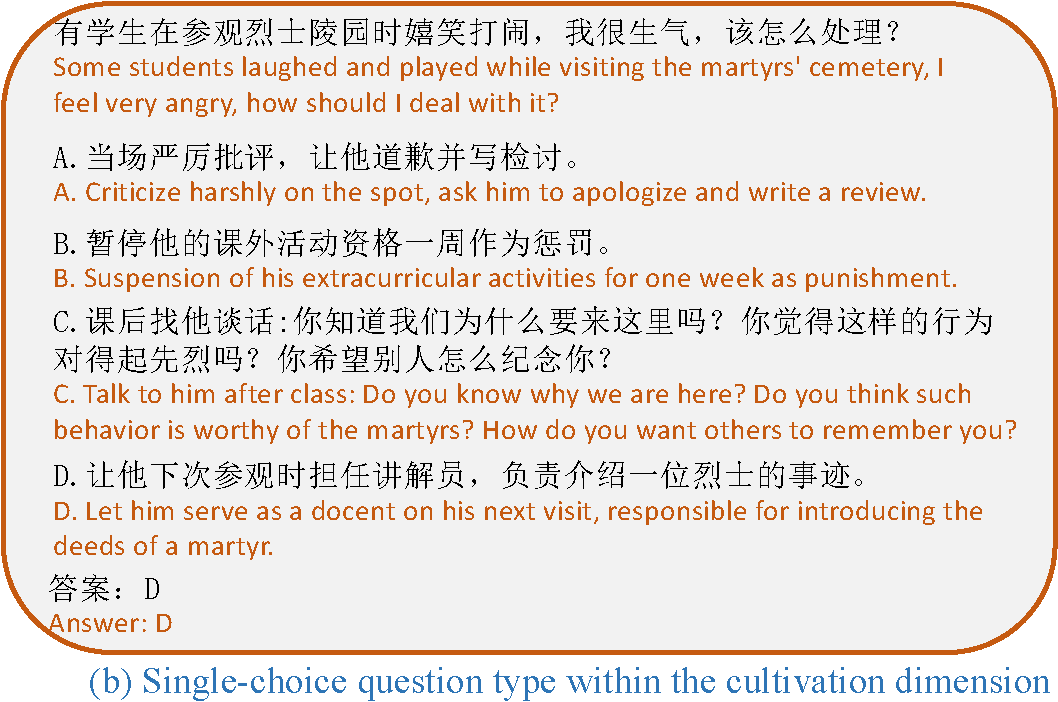
\includegraphics[height=0.32\textwidth]{figure/omni2.pdf}
    \vspace{-3mm}
    \caption{Example of (a) a single-choice question in the knowledge from a college chemist. (b) A single-choice question in the cultivation. English translations are shown for better readability.}
    \label{fig:omni12}
    \vspace{-3mm}
\end{figure}

\begin{figure}[tbp]
    \centering
    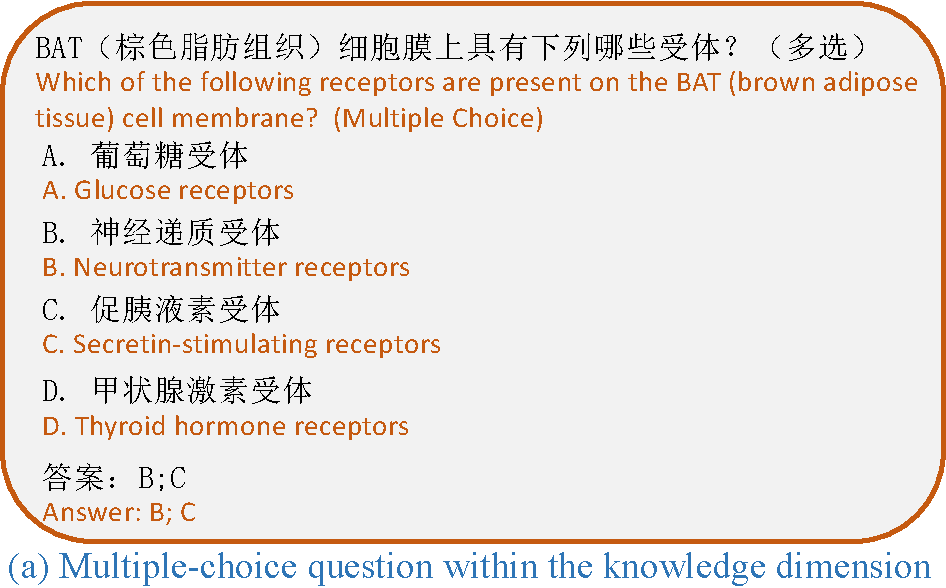
\includegraphics[height=0.3\textwidth]{figure/omni3.pdf}
    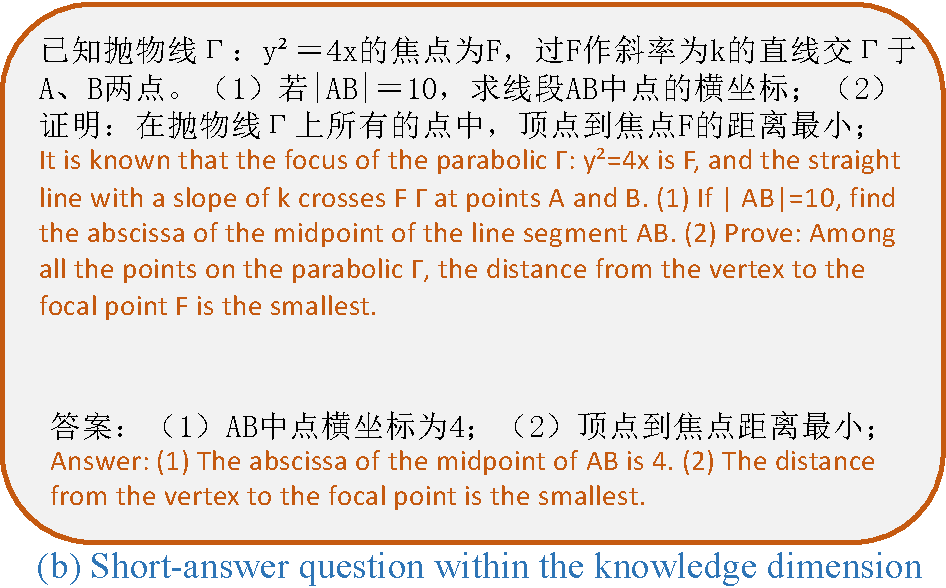
\includegraphics[height=0.3\textwidth]{figure/omni4.pdf}
    \vspace{-3mm}
    \caption{Example of (a) a multiple-choice question in the knowledge from Biology. (b) A short-answer question in the knowledge from Math. English translations are shown for better readability.}
    \label{fig:omni34}
    \vspace{-3mm}
\end{figure}





%%%基础教育
%在本研究中,我们首先通过在互联网上爬取和收集大量 K12 阶段的考试试卷,建立了一个较为完整的题库。为了便于后续处理和编辑,这些试卷数据经过 minerU 工具转化为 Markdown (md) 格式,从而实现结构化管理与信息的高效提取。

%在数据预处理环节,我们进一步对题目进行了分类与信息抽取,为每道题打上了多维度标签,包括 科目、学段以及题目类别。这一过程不仅使得题目能够更清晰地组织和索引,同时也为后续的数据分析与模型训练提供了必要的元信息支撑。

%为了保证题目的完整性与适用性,我们引入了 关键词过滤机制,用于检测题目及其对应解答是否依赖额外信息。例如,由于本研究所构建的数据集为单模态文本数据,并不包含图片信息,因此部分题目若在解答过程中需要图像、图表或公式等外部信息,则会通过关键词检索加以识别与剔除。这一策略有效降低了由于信息缺失而导致的题目不合理性。

%在构建题目与答案对应关系的过程中,我们利用 生成式大语言模型 (LLM) 对题目进行自动化解答匹配。然而,考虑到大模型在推理过程中存在一定的不确定性,其生成的答案可能与题意不符,甚至存在逻辑错误或事实性错误。为此,我们在后处理阶段引入了 闭源大模型作为校验器,对生成的题目与答案进行准确性和合理性检测,从而过滤掉了大量不符合标准的匹配结果。通过这一多层次的筛选流程,我们有效提升了数据集的质量与可靠性。

%整体而言,本研究构建的处理管线包括:数据爬取 → 格式转化 → 分类标注 → 关键词过滤 → 答案生成 → 准确性验证与筛选。这一系统化流程不仅确保了题目数据的规范性和科学性,同时也为后续的教育应用、智能出题与自动批改等场景奠定了坚实的基础。


%育人属性

%为系统评估生成式大语言模型(LLM)在 K12 场景下对关键“育人属性”的理解与迁移能力,本文基于公开可获得的教育类图书与学术论文构建场景化问答数据与相应评测协议。研究目标在于检验模型能否在真实教育情境中作出与价值导向一致、具有可执行性的判断与决策,而非仅停留在术语识别或模板化应答层面。

%数据构建首先从互联网收集与“育人”主题相关的书籍和论文,并对原始文本进行去重、清洗与结构化处理。在此基础上,提取“定义性描述”“干预策略与做法”“正反面案例”“可观察行为指标”等证据片段,形成可控生成所依托的素材池。随后依据“能力—情境—策略—行为表现”等维度对语料进行主题聚类,既保证内容的理论锚定与可追溯性,又为后续的场景重写与题项约束提供精确的证据支撑。

%在理论梳理和语料校对的基础上,本文将“育人”维度划分为二十个可操作属性:成长型思维、创新与创造力、反馈的建设性与及时性、反思性学习引导、个性化学习路径、批判性思维、情绪调控能力、启发式教学、社会责任感、同理心与共情、团队协作能力、问题解决能力、兴趣驱动学习、心理韧性与抗挫力、有效沟通能力、元认知能力、责任感与担当、正直与诚信、知识迁移能力、自信心与自我效能感。每个属性均提供简要定义、典型正向行为表现、易混淆的邻近概念与误用情形,以及可迁移的应用情境(课堂、家庭、社团、线上协作等),以此作为题项生成与评价的明确锚点。

%题项生成采用“证据驱动的场景重写—问项生成—答案约束”的流程。首先构建情境原型,明确角色(教师/学生/家长/同伴)、环境(学科或活动类型、线上/线下)、约束(时间、资源、评价压力)与目标(认知、情感、社会性)。其次完成属性对齐,为每个场景设定一个主属性及一至两个次属性,并在题干中避免显式暴露属性名称以减少词面提示与启发效应。随后指引 LLM 在限定的证据片段内生成题干、标准答案与简短判据,使答案体现“策略—因果链—预期结果”的可执行性与场景一致性,同时根据小学/初中/高中进行词汇难度与社会情境复杂度的年段适配。鉴于本研究数据为单模态文本形态,题项设计不依赖图片或图表信息,确保在无外部多模态资源时亦可完成作答。

%为检验模型对属性内涵的真正理解,本文为每个题项系统设计高迷惑度干扰项。干扰项刻意呈现“表层合理但情境失配”的特征,或在概念上与目标属性邻近却在要义上偏离(如反馈缺乏具体性或时效性),亦或提供短期有效但长期失衡的做法(例如立竿见影却削弱内在动机、诚信或协作),并在必要时设置触及教育伦理与安全红线的选项用于价值底线辨识。通过这类“部分正确但不符合场景”的设定,评测能够区分术语命中与真正理解。

%质量控制采取自动与人工相结合的策略。自动化阶段使用闭源校验模型对“题干—标准答案—理据”的一致性与价值合规性进行审查,剔除逻辑断裂与价值冲突样本,同时开展关键词泄露检测以避免目标属性或强提示词出现在题干中。必要时辅以具教育背景的人审抽检,对样本进行“一致/存疑/剔除”的标注并统计一致性指标;在试测基础上对题项进行难度标定,形成易/中/难分层,既便于后续实验设计,也有助于分析模型在不同难度水平上的表现差异。

%评测协议以多项选择题为载体,采用准确率作为核心指标,并以“标准答案与最强干扰项间的胜率差”衡量区分度,以检验干扰项的有效性与题项的辨析力。在模型可提供置信度的情况下,进一步计算 Brier 分数或期望校准误差以评估校准度。除总体结果外,报告分属性表现与跨场景的一致性,以检验模型在不同教育情境中的鲁棒性,并对各属性的题量、难度与通过率进行分布均衡性分析,防止由数据分布不均带来的结论偏置。

%该方案与本文前述的学科题库处理流水线保持兼容:从爬取与格式转化、分类标注、关键词过滤,到题目—答案的生成与闭源模型校验,均可复用统一的工程化组件。所有样本均绑定属性标签、年段、场景与角色等元数据,以支持高效检索与细粒度分析。研究全程遵循未成年人保护原则与学术伦理规范,避免刻板印象与歧视性表述;对于涉及心理与情绪的情境采用非伤害性语言;在数据使用与发布环节遵从版权与引用要求,尽可能实施最小必要摘录与重写,并移除可识别个人信息,同时对价值判断标准的理论来源予以说明,以提升研究的透明度与可复现性。


% 高等教育数据集处理过程
% 基于我们的调研,在目前的公开数据集中,中国高等教育习题的数据是广泛欠缺的。我们参照中国教育部普通高等学校本科专业目录,收集了涵盖哲学、教育学、法学、教育学、文学、历史学、理学、工学、农学、医学、军事学、管理学、艺术学这十三个学科大类的大量的中国高等教育复习资料、考研习题,并整理形成了我们的数据集。然而,这些习题大部分以PDF的形式存在,我们借助了MinerU提取工具从中解析出文字,并整理形成我们的高等教育题目数据集。为了保证题目的质量,我们进行了人工质检,筛除掉了识别混乱、语义不过关的题目。同时,为了确保题目的难度,我们采用了开源模型(Qwen-72B)进行了一轮答题,仅筛选了Qwen-72B答错并认为有挑战性的题目,以此保证了数据集中的题目对于大语言模型而言,是非常具有挑战性的。

% [1] 中国教育部普通高等学校本科专业目录:http://www.moe.gov.cn/srcsite/A08/moe_1034/s4930/202403/W020240319305498791768.pdf
% [2]MinerU: An Open-Source Solution for Precise Document Content Extraction 
% (https://arxiv.org/abs/2409.18839)

